\chapter{Main Modules}
\label{chTutorial}

The BATS agent architecture consists of several parts and layers. This tutorial guides you through using these parts step by step. All lower layers are independent of the higher layers, so if you do not need all layers, you can skip the later sections. For instance, if you are only interested in an easy interface with the simulation server, reading section \ref{secSocketComm} will suffice. If you want to start quickly with a working agent, you can skip until section \ref{secHumanoidAgent} for now. However, the agent template described there is based on the elements described in the sections before that, so be sure to read those too at some time, to fully understand how your agent works.

\begin{figure}
	\centering
	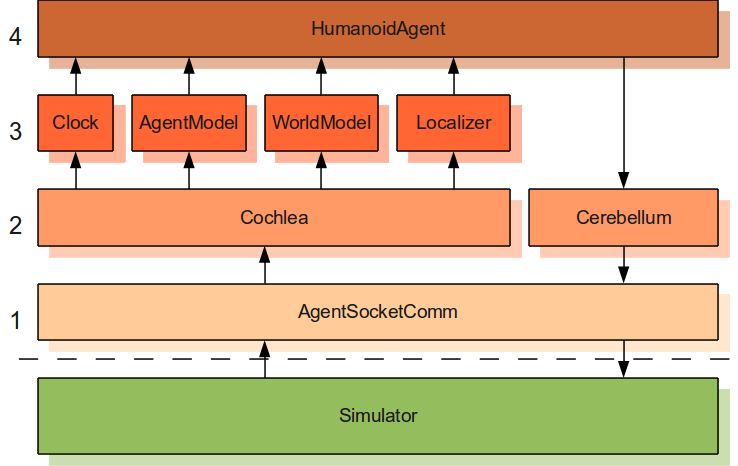
\includegraphics[width=0.7\textwidth]{libbats.png}
	\caption{{\tt libbats} modules}
	\label{fig:libbats}
\end{figure}

The main {\tt libbats} modules and their relations are shown in Fig.~\ref{fig:libbats}. As you can see, they can be divided into several layers:
\begin{description}
\item[1: Low level communication] As discussed in chapter \ref{chSimspark}, communication between the simulator and an agent is done using an ASCII, S-expression based protocol through a TCP/IP connection. The {\tt AgentSocketComm} module handles setting up this connection, reading and writing messages, and parsing these messages into and from more managable data structures. 
\item[2: Input and output integration] In the second layer, input and output is handled at a slightly higher level. On the input side, the {\tt Cochlea} extracts all data from the still text-based messages supplied by the {\tt AgentSocketComm} and turns that data into readily usable binary values. The {\tt Cerebellum} is used to gather control commands, work out contradictions if necesary and turn them into the text based structures that the {\tt AgentSocketComm} understands.
\item[3: Models] The 4 modules in the third layer use the data from the {\tt Cochlea} to update models of the current state of the world, i.e. the current time, the state of the agent's body, the state of the world and the game, and the location of all objects in the field.
\item[4: Intelligence] Finally, at the highest level, the actual intelligence of the agent is implemented. An instance of {\tt HumanoidAgent} has access to all information gathered in the different modules, decides upon actions based on this information, and submits these actions to the {\tt Cerebellum}.
\end{description}

In the following sections we will describe in more detail how each module can be used. While doing so, we will encounter different helper and utility classes. Please refer to later chapters for more details on these. Also, again, for more information, make sure to read the Doxygen documentation contained in the source.

\lstset{numbers=none}

\section{AgentSocketComm}
\label{secSocketComm}

\lstset{numbers=none}

As mentioned earlier, the lowest layer in the library manages the communication with the simulation server. This communication is done through TCP sockets and consists of S-expressions (predicates) that the agent and server send back and forth. To make sure you don't have to worry about what this stuff actually is and does, the library offers you the {\tt AgentSocketComm}. This class handles the connection to the server and sending, receiving and parsing of messages. This section explains how to use this module. If you use the {\tt HumanoidAgent} class, all this is done for you.

Before you can use {\tt AgentSocketComm}, you have to supply a host name and a port number to connect to. When running the server on the same computer as your agent, with default settings, these are 'localhost' and '3100'. After this is done, the first thing to do is to open an actual connection by calling {\tt connect()}:
\begin{lstlisting}[frame=single]
AgentSocketComm& comm = SAgentSocketComm::getInstance();
comm.initSocket("localhost", 3100);
comm.connect();
\end{lstlisting}

Note that the {\tt AgentSocketComm} is a singleton, refer to later chapters for information on what this is. The {\tt AgentSocketComm} keeps two internal message queues, one for input and one for output. These queues are filled and emptied, respectively, when calling {\tt AgentSocketComm}'s {\tt update()} method. This call blocks until new data is received from the server:
\begin{lstlisting}[frame=single]
comm.update();
\end{lstlisting}

SocketComm supplies several methods to place messages that should be sent to the server into the output queue. First of all, you can build your own predicate using the {\tt Predicate} and/or {\tt Parser} classes \footnote{This method is not described in this manual. Look at the documentation of the respective classes for more info} and put it directly into the queue by calling the send method:
\begin{lstlisting}[frame=single]
rf<Predicate> myPredicate = makeMyPredicate();
comm.send(myPredicate);
\end{lstlisting}
However, you can also leave the trouble of building the predicates to {\tt AgentSocketComm} by using its {\tt make*Message()} methods. And if you want it totally easy, use the {\tt init()}, {\tt beam()} and {\tt move*()} methods, which not only build the predicates, but also place the messages directly into the queue for you.

The input queue holds the messages received from the server. To check whether there is a new message, you can call {\tt hasNextMessage}. To extract the next message, you can use {\tt nextMessage()}:
\begin{lstlisting}[frame=single]
while (comm.hasNextMessage())
  rf<Predicate> message = comm.nextMessage();
\end{lstlisting}

To conclude and summarize this section, a typical way to have successful communication with the server is presented here:
\begin{lstlisting}[frame=single]
// Get the AgentSocketComm, initialize and connect
AgentSocketComm& comm = SAgentSocketComm::getInstance();
comm.initSocket("localhost", 3100);
comm.connect();

// Create robot model
rf<Predicate> scene = new Predicate("scene");
scene->pushLeaf("rsg/agent/" + am.getRSG());
comm.send(scene);

// Wait for the first message from the server
comm.update();

// Identify yourself to the server
comm.init(0, "MyTeam");

// Main loop
while (true)
{
  comm.update();
  while (comm.hasNextMessage())
    handleMessage(comm.nextMessage());
}
\end{lstlisting}

\section{Cochlea}
\label{secCochlea}

\lstset{numbers=none}

The {\tt AgentSocketComm} parses the S-expressions that the agent receives from the server into a {\tt Predicate} structure. However, to extract useful data you still have to dig through these structures. The {\tt Cochlea} offers a layer over the {\tt AgentSocketComm} to extract information from the predicates received from the server and present it in an easily accessible way.

Before using the Cochlea you have to initialize some parameters. You have to let it know what the name of your team is, so it can tell team mates and opponents apart:
\begin{lstlisting}[frame=single]
Cochlea& cochlea = SCochlea::getInstance();
cochlea.setTeamName("MyTeam");
\end{lstlisting}

Next you have to set up translations for joint-angle sensors. The {\tt Cochlea} uses internal names for these, that may not be the same as the names used in the messages sent by the server. These internal names are "head1", "head2", "larm1" to "larm4" for the left arm, "rarm1" to "rarm4" for the right and "lleg1" to "lleg6" and "rleg1" to "rleg6" for the legs. The Nao robot used by the server for instance uses names of the form "laj1" and "rlj3", so these have to be translated:
\begin{lstlisting}[frame=single]
cochlea.setTranslation("laj1", "larm1");
cochlea.setTranslation("rlj3", "rleg3");
\end{lstlisting}
This way the Cochlea can handle different robot models. If you use the {\tt AgentModel} module, this is done for you.

Now you can start using the {\tt Cochlea} by calling {\tt update()} every time a new message is received by the {\tt AgentSocketComm}. This will integrate the information of the message, after which you can request data with the {\tt getInfo()} method, or one of the methods for more complex data:
\begin{lstlisting}[frame=single]
comm.update();
cochlea.update();
// Get the polar coordinates of the ball
Vector3D polarBallPos = cochlea.getInfo(
                          Cochlea::iVisionBall);
\end{lstlisting}

\section{Clock}
\label{secClock}

The {\tt Clock} is pretty straightforward: it tells the current time:
\begin{lstlisting}[frame=single]
double t = SClock::getInstance().getTime()
\end{lstlisting}

\section{AgentModel}
\label{secAgentModel}

The \\{\tt AgentModel} keeps a model of the agent's own state. It keeps track of joint angles and data of other sensors, as well as some higher level data, like the position of the Center Of Mass (COM). The {\tt AgentModel} also needs some initialization before it can be used. You have to tell it the uniform number of the agent, after which you should call the {\tt initBody()} method:
\begin{lstlisting}[frame=single]
AgentModel& am = SAgentModel::getInstance();
am.setUnum(unum);
am.initBody();
\end{lstlisting}

This loads an XML configuration file that contains the names, sizes and weights of the agent's body parts and joints. It also uses this data to set up the translations for the {\tt Cochlea} for you, so you don't have to do this by hand. If default settings are used, the default configuration file {\tt conf.xml} is loaded, which is installed with the library and which imports the {\tt nao\_mdl.xml} file for each agent to get the description of the Nao robot model. For more information on loading XML configuration files and the robot model descriptions, see the documentation of the {\tt Conf} class.

After initialization, the {\tt AgentModel} is also ready to be updated and used:
\begin{lstlisting}[frame=single]
comm.update();
cochlea.update();
am.update();

Vector3D com = am.getCOM();
\end{lstlisting}

\section{WorldModel}
\label{secWorldModel}

The raw data offered by the {\tt Cochlea} may not be directly usable and perhaps you want to have some information that is deduced from these facts. This is exactly what the {\tt WorldModel} is for. It for instance gives the current game state and field size, but also higher level information like which team should take the kick-off, or if there is another player closer to the ball.

To start, the {\tt WorldModel} also needs to know the name of your team for some of its capabilities:
\begin{lstlisting}[frame=single]
WorldModel& wm = WorldModel::getInstance();
wm.setTeamName("MyTeam");
\end{lstlisting}

Next, the model has to be updated at every cycle. The {\tt WorldModel} extracts data from the {\tt Cochlea}, so make sure it is updated before updating the {\tt WorldModel}:
\begin{lstlisting}[frame=single]
comm.update();
cochlea.update();
wm.update();

bool shouldWeKickOff = wm.weGetKickOff();
\end{lstlisting}

\section{Localizer}
\label{secLocalizer}

\begin{figure}
\centering
\subfigure[Agent]{
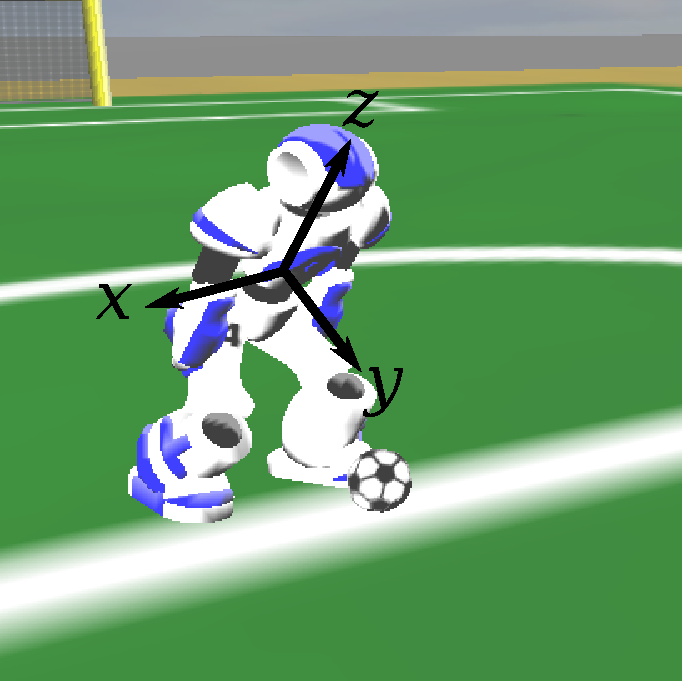
\includegraphics[width=.3\textwidth]{raw.pdf} \label{coordinatesraw}
}
\subfigure[Local]{
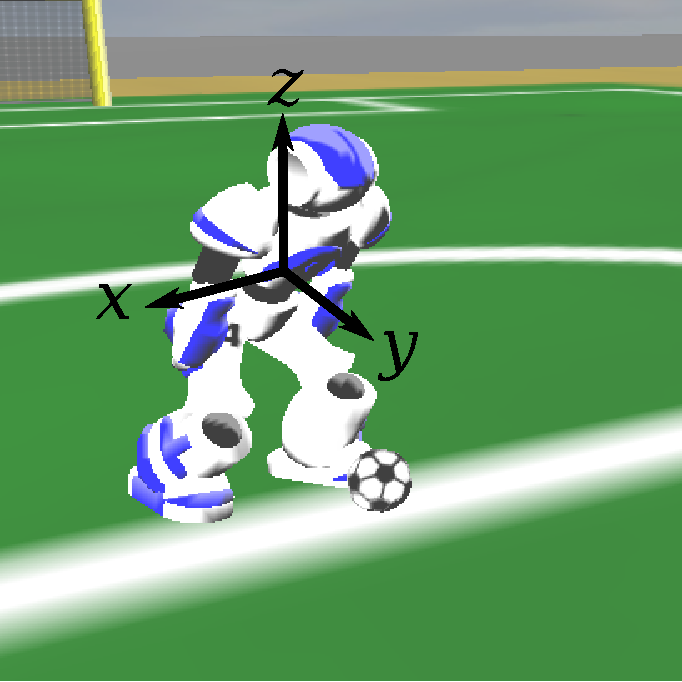
\includegraphics[width=.3\textwidth]{local.pdf} \label{coordinateslocal}
}
\subfigure[World]{
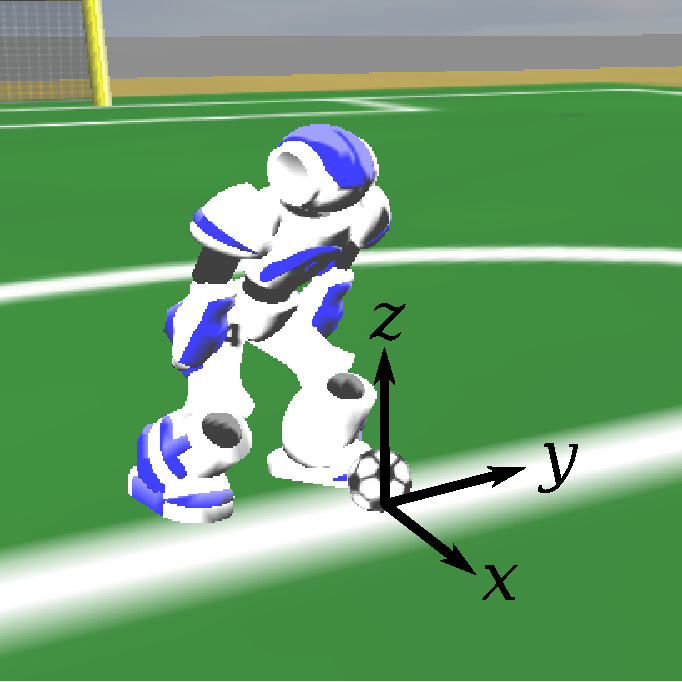
\includegraphics[width=.3\textwidth]{world.pdf}\label{coordinatesworld}
}
\caption{The coordinate systems used in {\tt libbats}: (a) Agent ('raw') coordinates, (b) local coordinates, and (c) global coordinates.}
\label{coordinates}
\end{figure}

The WorldModel provides the state of the game, such as the game time, the gamestate, and the team name. However, often the agents will want to know where they are, where the ball is, or where their opponents are. This can be obtained through the {\tt Localizer}. To be able to implement different localization methods, the {\tt Localizer} is an abstract class from which all implementations are derived. One realization of this class is provided in {\tt libbats}, called the {\tt KalmanLocalizer}. As you might have guessed, this {\tt Localizer} uses a Kalman filter to keep track of the locations of the player itself and of other objects. At the start of the program, we have to initialize the Localizer and tell it which implementation to use:
\begin{lstlisting}[frame=single]
SLocalizer::initialize<KalmanLocalizer>();
\end{lstlisting}

Like the other models, the update() member function of the {\tt Localizer} should be called each timestep to update the current location estimates with new data from the {\tt Cochlea}. The other member functions of the Localizer can be used to obtain the current position of the agent itself, the ball, the other players, or objects such as the goal posts and corner flags.

Within {\tt libbats}, several different coordinate systems are used (see Fig.~\ref{coordinates}:
\begin{description}
\item[Agent/raw coordinates] The origin of this system is the center of the agent's torso. The positive x axis extends to the right, parallel to the line through the shoulders, the positive y axis forward out of the torso, and the positive z-axis upwards, through the center of the head. This system is used by the {\tt AgentModel} for the coordinates of body parts. Shown in Fig.\ref{coordinatesraw}.
\item[Local coordinates] The origin of the local coordinate system is also the center of the agent's torso, but the positive z axis of this system always points upwards, perpendicular to the field. So, the x and y axes always lie parallel to the field, pointing right and forward respectively. This is one of the systems used by the {\tt Localizer} and is the most intuitive to use to determine 'in front of me/to the side of me/above of me' relations. Shown in Fig.\ref{coordinateslocal}.
\item[World coordinates] The world coordinate system is fully independent of the agent's location and orientation. Its origin is the center of the field, the positive x axis points to the center of the opponent's goal, the positive y-axis to the left when looking along the x axis, and the positive z axis points up, perpendicular to the field. This is the second system that is used by the {\tt Localizer} and is the best one to use to determine global relations. Shown in Fig.\ref{coordinatesworld}.
\end{description}

\section{Cerebellum}
\label{secCerebellum}

The {\tt Cochlea} takes the trouble of having to deal with raw predicates on the input side. On the output side the {\tt Cerebellum} is there for you. It supplies more useful structures to define actions and the possibility to integrate actions from different sources in your agent. The {\tt Cerebellum} defines the {\tt Action} substructure and a few of its derivatives with which you can make new actions. At the moment there are 5 different action types available:
\begin{description}
\item[{\tt MoveJointAction}] Move a hinge joint or one axis of a universal joint.
\item[{\tt MoveHingeJointAction}] Move a hinge joint.
\item[{\tt MoveUniversalJointAction}] Move both axes of a universal joint.
\item[{\tt BeamAction}] Beam to a certain position.
\item[{\tt SayAction}] Shout something.
\end{description}
If you don't understand the difference between hinge and universal joints, don't worry. Just use {\tt MoveJointAction}s and let the {\tt Cerebellum} handle the rest.

The {\tt Cerebellum} again is a singleton that can be retrieved by calling \\ {\tt SCerebellum::getInstance()}, after which you can add actions to it. After all the sub parts have added their actions, you can call {\tt outputCommands()} to send them through an {\tt AgentSocketComm}:
\begin{lstlisting}[frame=single]
Cerebellum& cer = SCerebellum::getInstance();

rf<MoveJointAction> action =
  new MoveJointAction(Types::LLEG1, 0.1);
cer.addAction(action);

cer.outputCommands(comm);
\end{lstlisting}
When more than one action is supplied for a joint, the angular velocities will be added together before sending the actions to the server.

\section{HumanoidAgent}
\label{secHumanoidAgent}

Now you have learned about how to initialize, update and maintain the several models of the library, you will learn how to forget all that. The {\tt HumanoidAgent} class does this all for you. It connects the {\tt AgentSocketComm}, initializes the {\tt Clock}, {\tt AgentModel}, {\tt WorldModel} and {\tt Localizer} and updates all modules in the correct order at every cycle. See chapter \ref{chQuickstart} to learn how to use this class to set up your own agent.

%\section{Behavior}
%\label{secBehavior}
%
%The code in the previous section implements an agent which connects to te server, gets placed in the field and then stands there until it falls over. Now it is time to let your agent behave. The BATS agent architecture supplies a hierarchical behavior model to help you with this by following these steps:
%
%\begin{itemize}
%\item Implement seperate behaviors
%\item Create a configuration file placing the behaviors in a hierarchical structure
%\item Create and run the behaviors
%\end{itemize}
%
%\subsection{Implementing a behavior}
%\label{subsecImplementingBehavior}
%
%The BATS agent architecture gives the {\tt Behavior} class as the building block of your agent. The basic thing to know is that a behavior receives a goal from a higher level behavior, creates subgoals that it wants to achieve in order to achieve the main goal and passes these goals to its subbehaviors. The behavior defines a sequence of slots in which arbitrary sub behaviors can be placed. This section shows how to create a behavior, section \ref{subsecConfiguration} will show how to define its super and sub behaviors.
%
%\subsubsection*{Inherit Behavior}
%
%The first thing to do when creating a new behavior is to create a class that inherits from the {\tt Behavior} class. It defines a couple of pure virtual methods that each behavior should implement (more on these later):
%
%\begin{program}
%\begin{verbatim}
%class MyBehavior : public Behavior
%{
%  virtual rf<Goal> generateGoal(unsigned step,
%                                unsigned slot);
%  virtual rf<State> getCurrentState();
%  virtual ConfidenceInterval getCapability(rf<State> s,
%                                           rf<Goal> g);
%
%public:
%  MyBehavior(std::string const &id,
%             std::string const &playerClass);
%};
%\end{verbatim}
%\end{program}
%
%You can do this by hand, but you can also use the utility script {\tt createbehavior.pl} to do this for you:
%
%\begin{program}
%\begin{verbatim}
%$ cd util/
%$ ./createbehavior.pl
%[Enter the behaviors name (e.g. MyBehavior)]
%\end{verbatim}
%\end{program}
%
%This creates a directory with your behavior's name in the Behavior directory and fills it with a header file with the necesary method declarations and code files with basic implementations for these methods.
%
%\subsubsection{Constructor (defining slots)}
%
%After making the base of your behavior you have to implement the constructor, where you define the structure of the behavior's sub behaviors by creating slots. The {\tt createbehavior.pl} script makes a start by creating a tree that defines a sequence of 1 step with 1 slot:
%
%\begin{program}
%\begin{verbatim}
%// Define the root, which is always a sequence:
%d_tree = new AST::Node(sequenceType);
%// Add one step to the sequence:
%d_tree->addChild(new AST::Node(andType));
%// Add one slot to the first step:
%d_tree->getChild(0)->addChild(new AST::Node(orType));
%\end{verbatim}
%\end{program}
%
%If you need more steps in the sequence, you can add new conjunction nodes ({\tt andType}) to the root, if you want to run sub behaviors in parallel in a step, you can add new disjunction nodes ({\tt orType}). The following gives an example of a behavior with 3 sequence steps and 2 parallel slots in the second step:
%
%\begin{program}
%\begin{verbatim}
%// Define the root, which is always a sequence:
%d_tree = new AST::Node(sequenceType);
%
%// Add first step to the sequence:
%d_tree->addChild(new AST::Node(andType));
%// Add one slot to the first step:
%d_tree->getChild(0)->addChild(new AST::Node(orType));
%
%// Add second step to the sequence:
%d_tree->addChild(new AST::Node(andType));
%// Add two slots to the second step:
%d_tree->getChild(1)->addChild(new AST::Node(orType));
%d_tree->getChild(1)->addChild(new AST::Node(orType));
%
%// Add third step to the sequence:
%d_tree->addChild(new AST::Node(andType));
%// Add one slot to the third step:
%d_tree->getChild(2)->addChild(new AST::Node(orType));
%\end{verbatim}
%\end{program}
%
%\subsubsection*{getCurrentState()}
%
%The first virtual method to implement is {\tt getCurrentState}. Different behaviors rely on different information of the world and/or agent state. In the BATS agent architecture a behavior defines this state itself in a standardized tree-based state description. This standardization is useful when using a learning algorithm to train different behaviors that use different state information. These state descriptions can also be used to define goals as states that should be reached, as we will see in the next sections.
%
%A basic state description is a conjunction of the state of several variables. To cater for uncertainty, the state of a variable is defined as a range of possible values:
%
%\begin{equation}
%\label{eqState}
%(0 \leq BallDist < 5) \wedge (10 \leq OpponentDist < 15)
%\end{equation}
%
%A behavior's state is defined in its {\tt getCurrentState} method. The {\tt createbehavior.pl} script sets up a conjunction for you to place variables into. The following code shows how to create the state in \ref{eqState}:
%
%\begin{program}
%\begin{verbatim}
%rf<State> state = new State();
%rf<OrNode> dis = state->addDisjunct();
%rf<AndNode> con = dis->addConjunct();
%
%con->addVar("BallDist", 0, 5);
%con->addVar("OpponentDist", 10, 15);
%\end{verbatim}
%\end{program}
%
%
%\subsubsection*{getCapability()}
%
%Behaviors that are placed in the same slot compete with each other for execution. They receive the same goal and are selected based on their capability to achieve that goal. Also, before advancing to the next sequence step, a behavior checks whether the sub behaviors in that step have enough capability to finish that step. A behavior's capability is requested by calling its {\tt getCapability} method, passing it a goal and the state it created in {\tt getCurrentState}. The behavior returns an estimate of its capability of achieving the goal, ranging from -1 to 1, with a confidence interval that depicts the accuracy of the estimate.
%
%\subsubsection*{Commitment}
%
%As explained earlier a behavior can commit to its goal when it is chosen. By doing so, it lets the super behavior know that it will take some time to reach the goal and that in intermediate steps it could not be good to switch between behaviors. Commitment is requested by setting the d\_committed member variable, which should be done in the behavior's overloaded {\tt update} method:
%
%\begin{program}
%\begin{verbatim}
%void MyBehavior::update()
%{
%  Behavior::update();
%  
%  // Check if we are already committed
%  // due to committed subbehavior(s)
%  if (d_committed)
%    return;
%  
%  // Commit if we can still reach our goal  
%  if (goalStillReachable())
%    d_committed = true;
%  else
%    d_committed = false;
%\end{verbatim}
%\end{program}
%
%The {\tt update} method is called at the beginning of each time step if the behavior could be selected to run that timestep. First of all the {\tt Behavior::update} should be called. This updates the child behaviors, checks if they are committed and commits the behavior if it should commit if children are committed \footnote{Abbreviated to SCICC (Should Commit If Children Commit)}. If this is the case you can choose to override this, but usually you just return.
%
%Next you check whether the behavior should commit to its goal. Usually this is the case when the goal can still be reached. It is important to also reset the flag when a goal is no longer reachable, as shown in the example, to prevent a behavior to lock the agent in useless behavior. Note that the behavior's goal ({\tt d\_goal}) is the goal received in the previous timestep.


%\subsection{Configuration XML setup}
%\label{subsecConfiguration}
%The humanoidbats agent has to have an XML configuration file. This file is used to structure all the behaviors in the binary together. The XML file will define all the steps and slots and will define a root behavior which is at the top of the behavior hierarchy.
%The general XML layout contains:
%%
%%
%%  HIERONDER MNOETEN NOG LINKS KOMEN NAAR DE HOOFDSTUKKEN..........
%%
%%
%%
%\begin{itemize}
%\item The root conf element
%	\item The player id (unum) to class type coupling
%	\item The player class defenitions
%\begin{itemize}
%		\item The behaviors element
%\begin{itemize}
%			\item Behavior elements
%\begin{itemize}
%				\item Behavior parameters
%				\item Behavior slots
%\end{itemize}
%\end{itemize}
%\end{itemize}
%\item XIncludes
%\end{itemize}
%
%\subsubsection*{The root conf element}
%Every XML file has a root element, in the configuration XML files this is the conf element. If the file includes other XML files, make sure to include the XInclude namespace. The most common header will therefore contain:
%
%\begin{program}
%\begin{verbatim}
%<?xml version="1.0" encoding="ISO-8859-1"?>
%
%<conf xmlns:xi="http://www.w3.org/2003/XInclude">
%\end{verbatim}
%\end{program}
%
%
%\subsubsection*{The player id (unum) to class type coupling}
%All the players on the field share the same XML configuration files as they are all instances of the same command. To allow for the different player types to share the same XML, the playerclass has been added. Every agent has a playerclass, and all player classes have their own behavior hierarchy. To define which player class is used for which unum, the following code is used:
%
%\begin{program}
%\begin{verbatim}
%<player id="1" class="attacker" />
%\end{verbatim}
%\end{program}
%
%
%\subsubsection*{The player class definitions}
%The player class element holds the behaviors for the player class. Every player class has an id and contains the behaviors.
%
%\begin{program}
%\begin{verbatim}
%<player-class id="attacker">
%\end{verbatim}
%\end{program}
%
%\subsubsection*{The behaviors element}
%The behaviors element is a simple container element for all the behavior elements. It currently has no attributes, but must contain at least one behavior with the id “win”.
%
%\subsubsection*{Behavior elements}
%The behavior elements contain all the information for the behavior structure. Every behavior has a type, that names the name of the behavior in the binary, and an unique id, which is used to reference it from other parts of the XML. The id only has to be unique within the behaviors parent element, not the whole configuration XML.
%
%\begin{program}
%\begin{verbatim}
%<behavior type="MyBehavior" id="mybehavior">
%\end{verbatim}
%\end{program}
%
%\subsubsection*{Behavior parameters}
%Behavior parameters are behavior specific and are used in by the binary behavior to make it more general in use.
%All parameters for a behavior are kept inside the \emph{param} element. This element can contain any type of element which is totally up to the binary behavior.
%An example of is:
%\begin{program}
%\begin{verbatim}
%  <param>
%        <deg>10</deg>
%        <joint slot="0">&rleg5;</joint>
%        <joint slot="1">&lleg5;</joint>
%  </param>
%\end{verbatim}
%\end{program}
%
%\subsubsection*{Behavior slots}
%Every behavior can have other behaviors below it. These other behaviors can be run in parallel, in sequence, or in competition.
%The slots are created with a \emph{slot} element which is a direct descendant of the behavior element. Each slot has an index attribute
%which describes where it is placed below the behavior. The first digit of the index indicates the step, and the second digit indicates the slot. Each slot, in turn, contains any number of references to behaviors defined in the
%configuration.
%
%Remember, steps are executed in sequence. Within steps, slots are executed in parallel, and within each slot only one of the alternative behaviors is chosen.
%
%To reference to a behavior, a \emph{behavior} element should be used with a \emph{refid} attribute containing the XML configuration id of the behavior.
%
%A typical example:
%
%\begin{program}
%\begin{verbatim}
%<slot index="0-0">
%  <behavior refid="alternativeA" />
%  <behavior refid="alternativeB" />
%  <!--either alternativeA or alternativeB is executed -->
%</slot>
%<slot index="0-1">
%  <behavior refid="parallelBehavior" />
%  <!--parallelbehavior is executed in parallel with 
%  either alternativeA or alternativeB-->
%</slot>
%<slot index="1-0">
%  <behavior refid="secondStep" />
%  <!--secondStep is done after all of the above -->
%</slot>
%\end{verbatim}
%\end{program}
%
%
%\subsection{Creating and Running Behaviors}
%
%Now you have defined all your behaviors and set up the hierarchy in your XML configuration file. The last thing to do is to have your agent create the correct behavior tree based on the configuration file and run the behaviors every time step. The first you simply do by loading the configuation file with the {\tt Conf} class and then call the static {\tt Behavior::createBehaviors} method:
%
%\begin{program}
%\begin{verbatim}
%void MyAgent::init()
%{
%  Conf::initialize("myconf.xml");
%  Behavior::createBehaviors();
%}
%\end{verbatim}
%\end{program}
%
%As you can see, your agent's {\tt init} method is a good place to do it. Running your behaviors consists of running the root behavior, which in its turn runs its subbehaviors, et cetera, until the lowest, primitive behaviors are run. Just select your root behavior (we like to call it the 'win' behavior and is the behavior with id 'win') and run it:
%
%\begin{program}
%\begin{verbatim}
%void MyBehavior::think()
%{
%  rf<Behavior> win = Behavior::getWin();
%  win->update();
%  win->setGoal(new Behavior::Goal);
%  win->achieveGoal();
%}
%\end{verbatim}
%\end{program}
%
%After the behavior tree is processed, the primitive behaviors that have actions to send to the server  are collected in the list of Action Command Behaviors. You should request these, collect their actions and send them to the Cerbellum:
%
%\begin{program}
%\begin{verbatim}
%void MyBehavior::think()
%{
%  ...
%  Cerebellum& cer = SCerebellum::getInstance();
%  
%  std::set<rf<Behavior> > acBehaviors = 
%      Behavior::getActionCommandBehaviors();
%  for (set<rf<Behavior> >::iterator iter = 
%          acBehaviors.begin(); iter != acBehaviors.end(); ++iter)
%  	cer.addAction((*iter)->getAction());
%  
%  cer.outputCommands(d_comm);
%}
%\end{verbatim}
%\end{program}
